\documentclass[a4paper, 12pt]{article}%тип документа

%отступы
\usepackage[left=2cm,right=2cm,top=2cm,bottom=3cm,bindingoffset=0cm]{geometry}
\setlength{\parindent}{5ex}

%Русский язык
\usepackage[T2A]{fontenc} %кодировка
\usepackage[utf8]{inputenc} %кодировка исходного кода
\usepackage[english,russian]{babel} %локализация и переносы

%Вставка картинок
\usepackage{graphicx}
\graphicspath{{pictures/}}
\DeclareGraphicsExtensions{.pdf,.png,.jpg}

%Графики
\usepackage{pgfplots}
\pgfplotsset{compat=1.9}

%Математика
\usepackage{amsmath, amsfonts, amssymb, amsthm, mathtools}

%Таблицы
\usepackage{longtable} 
\usepackage{float}

%Римские цифры
\newcommand{\RomanNumeralCaps}[1]{\uppercase\expandafter{\romannumeral#1}}

\usepackage{multirow}


\begin{document}
	\begin{titlepage}
		\begin{center}
			\textsc{Федеральное государственное автономное образовательное учреждение высшего образования«Московский физико-технический институт (национальный исследовательский университет)»\\[5mm]
			}
			
			\vfill
			
			\textbf{Отчёт по лабораторной работы 2.1.3\\[3mm]
				Определение $C_p / C_v $ по скорости звука в газе.
				\\[50mm]
			}
			
		\end{center}
		
		\hfill
		\begin{minipage}{.5\textwidth}
			Выполнил студент:\\[2mm]
			Сериков Василий Романович\\[2mm]
			группа: Б03-102\\[5mm]
			
		\end{minipage}
		\vfill
		\begin{center}
			Москва, 2022 г.
		\end{center}
		
	\end{titlepage}
	
	\newpage
	
	\textbf{Аннотация}
	
	
	\paragraph{Цель работы:} 1) измерение частоты колебаний и длины волны при резонансе звуковых колебаний в газе, заполняющем трубу; 2) определение показателя адиабаты с помощью уравнения состояния идеального газа.
	\\
	
	\textbf{Теоретические сведения}
	
Cкорость распространения звуковой волны в газах зависит от показателя адиабаты $\gamma$. На измерении скорости звука основан один из наиболее  точных методов определения показателя  адиабаты.

Скорость звука в газах определяется формулой:
$$c=\sqrt{\gamma\frac{RT}{\mu}},$$
где $R$ - газовая постоянная, $T$ - температура газа, а $\mu$ его молярная масса. Выразим показатель адиабаты:
$$\gamma=\frac{\mu}{RT} c^2$$

Звуковая волна, распространяющаяся вдоль трубы, испытывает многократные отражения от торцов. Звуковые колебания в трубе являются наложением всех отраженных волн и, вообще говоря, очень сложны. Картина упрощается, если длина трубы L равна целому числу полуволн, то есть когда
$$L=n\frac{\lambda}{2},$$
где $\lambda$ — длина волны звука в трубе, а $n$ — любое целое число.

Скорость звука c связана с его частотой $f$ и длиной волны $\lambda$ соотношением:
$$c=\lambda f.$$

Подбор условий, при которых возникает резонанс, можно производить двояко:

1) При неизменной частоте f звукового генератора (а следовательно, и неизменной длине звуковой волны $\lambda$) можно изменять длину трубы $L$. Для этого применяется раздвижная труба. Длина раздвижной трубы постепенно увеличивается, и наблюдается ряд последовательных резонансов. Для $k$-ого резонанса имеем:
$$L_{n+k}=n\frac{\lambda}{2} + k\frac{\lambda}{2},$$
т. е. $\lambda/2$ равно угловому коэффициенту графика, изображающего зависимость длины трубы $L$ от номера резонанса $k$.

2) При постоянной длине трубы можно изменять частоту звуковых
колебаний. В этом случае следует плавно изменять частоту $f$ звукового генератора, а следовательно, и длину звуковой волны $\lambda$.
Для $k$-ого резонанса получим:
$$L = (n+k)\frac{\lambda_{k+1}}{2}$$
$$f_{k+1} = \frac{c}{\lambda_{k+1}}=\frac{c}{2L}(n+k)=f_1 + \frac{c}{2L}k.$$

Скорость звука, деленная на $2L$, определяется, таким образом,
по угловому коэффициенту графика зависимости частоты от номера
резонанса.
	\\
	\newpage
	
	\textbf{Методика измерений}

	\begin{figure}[h]
	\center{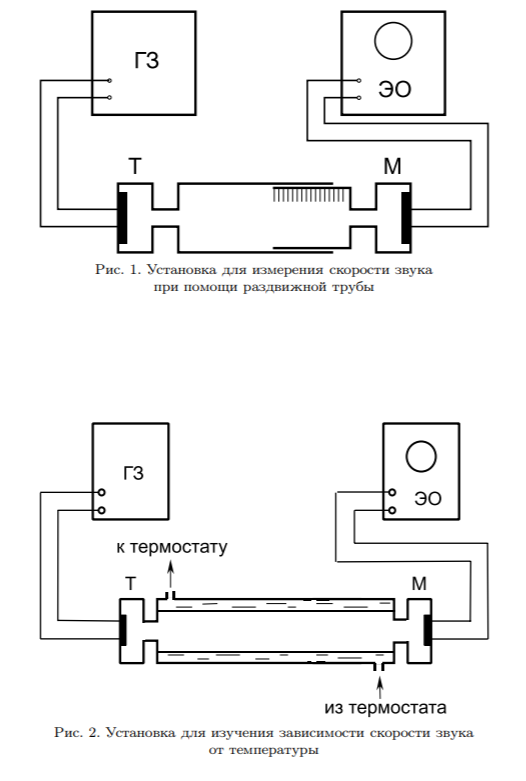
\includegraphics [scale=1]{ установка .png}}
\end{figure}
	
	
\textbf{Используемое оборудование:} 
звуковой генератор ГЗ; электронный осциллограф ЭО; микрофон; телефон; раздвижная труба; теплоизолированная труба, обогреваемая водой из термостата; баллон со сжатым углекислым газом; газгольдер.
	\\
	
\textbf{Результаты измерений и обработка данных: }	
	\paragraph { Измерение коэффициента $C_p / C_v $ для воздуха при помощи установки с раздвижной трубой.}
\begin{enumerate}
	\item Размеры установки и погрешности: $L  = 570 \pm 5$ мм, $\sigma_{\Delta l} =\pm 1$ мм.
	\item При постоянной начальной частоте будем находить точки резонанса для воздуха, увеличивая и уменьшая длину трубы. Полученные данные занесем в таблицу.
	\item По полученным данным построим графики зависимости $\Delta l (n)$. Коэффициент наклона прямой -- это величина $\lambda/2$. Тогда скорость звука можно найти по формуле: $c = \lambda f$, $\sigma_c=c\sqrt{(\frac{\sigma_f}{f})^2+(\frac{\sigma_{\lambda}}{\lambda})^2}$
	\newpage
	\begin{longtable}{|c|c|c|c|c|c|c|c|c|}
		\hline
		$ f $, кГц & \multicolumn{2}{c|}{\textbf{5}} & \multicolumn{2}{c|}{\textbf{4,5}} & \multicolumn{2}{c|}{\textbf{4}} & \multicolumn{2}{c|}{\textbf{3,5}} \\ \hline
		$ n $ & $\Delta l_n $, мм & $ \Delta l_n $, мм & $ \Delta l_n $, мм & $ \Delta l_n $, мм & $ \Delta l_n $, мм & $ \Delta l_n $, мм & $ \Delta l_n $, мм & $ \Delta l_n $, мм  \\ \hline
		1 & 23 & 21 & 10 & 10 &  &  &  &   \\ \hline
		2 & 57 & 57 & 48 & 48 & 38 & 39 & 25 & 25 \\ \hline
		3 & 91 & 91 & 87 & 86 & 83 & 82 & 75 & 74  \\ \hline
		4 & 126 & 125 & 125 & 124 & 124 & 123 & 123 & 128 \\ \hline
		5 & 160 & 160 & 163 & 167 & 167 & 173 & 173 & 171  \\ \hline
		\caption{Результаты измерений для воздуха}
	\end{longtable}
	
		\begin{figure}[h]
	    \center{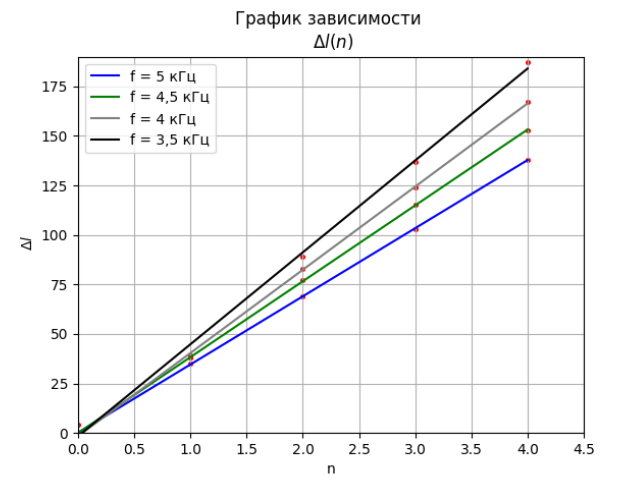
\includegraphics [scale=1]{air.png}}
		\caption{}
	    \end{figure}
    
    \begin{longtable}{|c|c|c|c|c|}
    	\hline
    	$ f $, кГц & $ \lambda $, мм & $ \sigma_\lambda $, мм & $ c $, м/с & $ \sigma_c $, м/с \\ \hline
    	5 & 68,8 & 0,2 & 344 & 1 \\ \hline
    	4,5 & 76,6 & 0,3 & 345 & 1 \\ \hline
    	4 & 85,0 & 0,3 & 340 & 1 \\ \hline
    	3,5 & 97,8 & 0,4 & 342 & 1 \\ \hline
    	\caption{Результаты вычислений для воздуха}
    \end{longtable}
    \item Получим среднее значение скорости звука в воздухе $c = (343 \pm 2)$ м/с
    \item Посчитаем коэффициент $\gamma = C_p / C_v $. $\gamma = \frac{\mu}{RT}c^2 $ 
    
    $\gamma = 1,387 \pm 0,006$
    \\

    \textbf{Измерение коэффициента $C_p / C_v $ для углекислого газа при помощи установки с раздвижной трубой.}
    
	\item Проведем измерения аналогичные измерениям $\gamma$ для воздуха. Полученные данные занесем в таблицу.
		\begin{longtable}{|c|c|c|c|c|c|c|c|c|}
		\hline
		$ f $, кГц & \multicolumn{2}{c|}{\textbf{5}} & \multicolumn{2}{c|}{\textbf{4,5}} & \multicolumn{2}{c|}{\textbf{4}} & \multicolumn{2}{c|}{\textbf{3,5}} \\ \hline
		$ n $ & $\Delta l_n $, мм & $ \Delta l_n $, мм & $ \Delta l_n $, мм & $ \Delta l_n $, мм & $ \Delta l_n $, мм & $ \Delta l_n $, мм & $ \Delta l_n $, мм & $ \Delta l_n $, мм  \\ \hline
		1 & 10 & 18 & 22 & 32 & 17 & 18 & 24 & 28  \\ \hline
		2 & 41 & 46 & 56 & 63 & 46 & 39 & 62 & 72 \\ \hline
		3 & 70 & 74 & 90 & 95 & 80 & 82 & 105 & 113  \\ \hline
		4 & 97 & 102 & 123 & 126 & 124 & 150 & 123 & 154 \\ \hline
		5 & 126 & 126 & 165 & 165 & 157 & 161 & 195 & 195  \\ \hline
		\caption{Результаты измерений для $CO_2$}
	\end{longtable}
	\item Аналогично при постоянной начальной частоте будем находить точки резонанса для углекислого газа и построим графики $\Delta l (n)$.
	
		\begin{longtable}{|c|c|c|c|c|}
			\hline
			$ f $, кГц & $ \lambda $, мм & $ \sigma_\lambda $, мм & $ c $, м/с & $ \sigma_c $, м/с \\ \hline
			5 & 55,1 & 0,4 & 275 & 1 \\ \hline
			4,5 & 61,3& 0,4 & 275 & 1 \\ \hline
			4 & 67,5 & 0,3 & 270 & 1 \\ \hline
			3,5 & 78,9 & 0,3 & 273 & 1 \\ \hline
			\caption{Результаты вычислений для $CO_2$}
		\end{longtable}
	
	\begin{figure}[h]
		\center{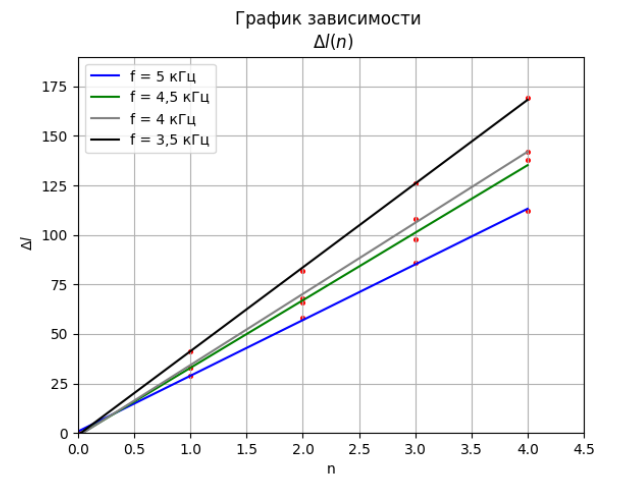
\includegraphics [scale=0.95]{co2.png}}
		\caption{}
	\end{figure}
	
    \item Получим среднее значение скорости звука в $CO_2$ $c = (273 \pm 2)$ м/с
	\item Посчитаем коэффициент $\gamma = C_p / C_v $. $\gamma = \frac{\mu}{RT}c^2 $ 
	
	$\gamma = 1, 333 \pm 0,004$
	\\
	 
	\textbf{Измерение $C_p / C_v $ при различных температурах воздуха}
	\item Начальные данные и погрешности: $L = 800 \pm 1$ мм
	\item Для постоянной температуры будем изменять частоту звука (изменяя и длину волны) так, чтобы наблюдались резонансы. Для полученного резонанса будем отмечать частоту, при которой он возник. Данные занесем в таблицу.

	\begin{longtable}{|c|c|c|c|c|c|c|c|}
		\hline
		$ t $,$^{\circ}C$  & \textbf{23,5} & \textbf{30} & \textbf{35} & \textbf{40} & \textbf{45} & \textbf{50} & \textbf{52}\\ \hline
		n &  \multicolumn{7}{c|}{$ f_n $, Гц } \\ \hline
		1 & 200 & 202  & 203  & 205 & 206 & 207 & 209 \\ \hline
		2 & 450  & 454  & 457  & 460  & 463 & 466 & 467 \\ \hline
		3 & 660  & 666  & 670  & 675  & 680 & 684 & 686 \\ \hline
		4 & 874  & 882  & 888 & 894 & 901 & 906 & 908 \\ \hline
		5 & 1088 & 1099  & 1106 & 1114  & 1122 & 1129 & 1133\\ \hline
		6 & 1305 & 1317 & 1327 & 1336 & 1346 & 1355 & 1358  \\ \hline
		7 & 1521  & 1536 & 1547 & 1558 & 1570 & 1579 & 1583 \\ \hline
		\caption{Результаты измерений частоты}
	\end{longtable}

\item По полученным данным построим графика зависимости $f_n (n)$. Коэффициент наклона прямой -- это величина $c / 2L$. Выразим скорость звука и полученные данные занесем в таблицу.

	\begin{figure}[h]
	\center{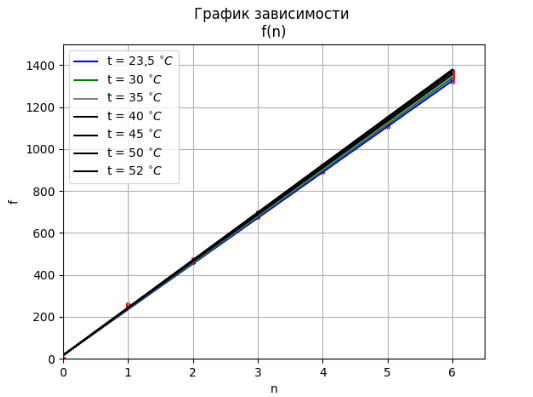
\includegraphics [scale=1]{temp.png}}
\end{figure}
\newpage

\begin{longtable}{|c|c|c|}
	\hline
	$ t $, $^{\circ}C$  & $ c $, м/с & $ \sigma_c $, м/с  \\ \hline
	23,5 & 348 & 1 \\ \hline
	30 & 352 & 1  \\ \hline
	35 & 353 & 1 \\ \hline
	40 & 356 & 1  \\ \hline
	45 & 360 & 1 \\ \hline
	50 & 362 & 1  \\ \hline
	52 & 362 & 1  \\ \hline
	\caption{Скорость звука при различных температурах}
\end{longtable}
 \item Получим среднее значение скорости звука в воздухе $c = (355 \pm 2)$ м/с
\item Посчитаем коэффициент $\gamma = C_p / C_v $. $\gamma = \frac{\mu}{RT}c^2 $ 

$\gamma = 1,485 \pm 0,004$
\end{enumerate}	


	\textbf{Обсуждение результатов:}
	Проведя измерения на двух установках мы получили значения скорости звука для воздуха, которые практически совпадают и соответствуют табличному значению, полученная нами скорость звука в углекислом газе выше табличной, скорее всего это связано с попаданием воздуха в установку. Соответственно показатель адиабаты в случае с воздухом близок к табличному, а в случае с углекислым газом не соответствует  действительности.
	
	
	\textbf{Выводы: }
	В ходе данной работы мы измерили частоты колебаний и длины волны при резонансе звуковых колебаний в газе. Определили показатели адиабаты с помощью уравнения состояния идеального газа.
	
	
	
	
	
	
	

\end{document}